\chapter{Orthogonality %, Orthogonal Projections 
and the Gram-Schmidt Algorithm}
\label{chapter:orthog}


So far, in all our generalizations of vectors spaces from $\R^2$ and
$\R^3$, we have not used the geometry of the dot product.  In this
section, we want to see what that extra geometry gives us, in 
the case of $\R^n$.  

In fact, one can add the extra geometry of
an inner product to any vector space; on spaces of (continuous) functions with
domain $[a,b]$, for example, the ``correct'' replacement to the
dot product of vectors is the following \stress{inner product} of functions:
$$
\langle f, g \rangle = \int_a^b f(x)g(x)\;dx
$$
This is a topic that you get to explore in second year analysis. One can also give a natural inner product  to spaces of matrices $\M_{m\, n}$ by the formula 
$$
\langle A, B \rangle = \tr (AB^T)
$$

The dot product and the above inner products have a number of 
extremely nice properties; but there are other \stress{bilinear forms}
that encode different geometries (such as space-time) more accurately.
You can explore this topic in more detail in 3rd year applied linear
algebra.



\section{Orthogonality}

Recall that two vectors $\uu, \vv \in \R^n$ are said to be \defn{orthogonal} if their
dot product $\uu \cdot \vv$ is zero.  The dot product satisfies:
\begin{itemize}
\item $\uu \cdot \uu \geq 0$ and is equal to zero iff $\uu = \zero$
\item $\uu \cdot \vv = \vv \cdot \uu$ (symmetry)
\item $(a\uu + b\vv)\cdot(c\ww) = ac \uu \cdot \ww + bc \vv \cdot \ww$
for all $a,b,c\in\R$ and $\uu,\vv,\ww \in \R^n$  and similarly
\item $(a\uu) \cdot (b\vv + c\ww) = ab\uu \cdot \vv + ac \uu \cdot \ww$
(bilinearity).
\end{itemize}
\begin{myexample} The vectors $(1,-1,0,1)$ and $(1,1,1,0)$ in $\R^4$ are orthogonal, since 

$$(1,-1,0,1)\cdot(1,1,1,0)=1\cdot 1 + (-1) \cdot 1 + 0\cdot 1 + 1 \cdot 0=1-1=0.$$

\end{myexample}

Note that the standard basis of $\R^3$, namely $\set{(1,0,0), (0,1,0), (0,0,1)}$ (or $\set{\ee_1, \ee_2, \ee_3}$) consists of vectors that are all pairwise orthogonal:  that is, 
$
\ee_i \cdot \ee_j = 0
$ for $ i\not=j$.

 We'd like to generalize this idea, since this basis has (at least) one very convenient property: for any $\vv \in \R^3$, it's easy to find $a,b$ and $c$ such that $\vv= a \,\ee_1 +b\,\ee_2+ c\,\ee_3$: we all know that $a=\vv\cdot \ee_1, b=\vv\cdot \ee_2$ and $c=\vv\cdot \ee_3$.


\section{Orthogonal sets of vectors}


\begin{definition}
A set of vectors $\{\vv_1, \cdots, \vv_m\}$ in $\R^n$ is called \defn{orthogonal} \index{orthogonal vectors} if
 $$
\vv_i \cdot \vv_j = 0
$$
for all $1 \leq i < j \leq m$, and $\vv_j\not=0$ for  all $1 \leq i  \leq m$. That is, every pair of vectors is orthogonal and no vector is zero.
\end{definition}

Note: If an orthogonal set consists of vectors all of which have length $1$, we call the set {\it orthonormal}. Indeed, if $\{\vv_1, \cdots, \vv_m\}$  is  orthogonal, then 
$\{\frac{\vv_1}{\|\vv_1\|}, \dots, \frac{\vv_m}{\|\vv_m\|}\}$ is orthonormal.


\begin{myexample} The standard basis of $\R^n$ is an orthogonal set. (It's also orthonormal.)\end{myexample}

\begin{myexample} $\{ (1,0,0), (0,1,0), (1,0,1)\}$ is NOT ORTHOGONAL even though two of the
products are zero --- since the first and third vectors aren't orthogonal, this
is not an orthogonal set. \end{myexample}

Orthogonal sets of vectors also enjoy a general Pythagorean property: if $\{\vv_1, \cdots, \vv_m\}$ is orthogonal, then 
\begin{equation*} \|\vv_1 + \vv_2 +\cdots + \vv_m\|^2 =\|\vv_1\|^2 + \|\vv_2\|^2 +\cdots + \|\vv_m\|^2 \tag{$\star$}\label{eqn:Pythag}
\end{equation*}
Prove this for yourself, remembering that $\|\vv\|^2= \vv\cdot \vv$.

Even better, (and just like the standard basis of $\R^n$) every orthogonal set is linearly independent:

\begin{theorem}[Linear independence of orthogonal sets]\index{linear independence of orthogonal sets}\label{theorem:orthogLI}
Any orthogonal set of  vectors is linearly independent.
\end{theorem}

\begin{proof}
Let $\{\vv_1, \cdots, \vv_m\}$ be an orthogonal set and 
suppose there are scalars $a_1, \dots a_m$ such that
$$
a_1\vv_1 + \cdots + a_m\vv_m = \zero.
$$
Take the dot product of both sides with $\vv_1$; the answer has to 
be zero because the right hand side is $\vv_1 \cdot \zero = 0$.  But on the left hand
side, we get
$$
\vv_1 \cdot (a_1\vv_1 + \cdots + a_m\vv_m) = a_1 \vv_1 \cdot \vv_1 + a_2 0 + \cdots +a_m 0
$$
since $\vv_1 \cdot \vv_j = 0$ for all $j>1$.  Since $\vv_1 \cdot \vv_1 \neq 0$
(since we assumed $\vv_1 \neq \zero$) we deduce that $a_1 = 0$.
Continuing in this way with each of the vectors gives $a_i=0$ for
all $i$, so this set is indeed linearly independent.
\end{proof}

This is a marvelous and wonderful fact!  
It gives us
\begin{itemize}
\item Any orthogonal set of   vectors in $\R^n$ has at most $n$ elements.
\item  Any orthogonal set of $n$  vectors in $\R^n$ is a basis for $\R^n$, called an \defn{orthogonal basis}.
\end{itemize}
Furthermore, the proof gave us a  {\it very} easy way to calculate the
coordinates of a vector relative to an orthogonal basis.

\begin{theorem}[The Expansion Theorem: Coordinates relative to an orthogonal basis]\label{expansion}\index{coordinates relative to an orthogonal basis}
Suppose $\{\ww_1, \cdots, \ww_m\}$ is an orthogonal basis for a subspace $W$ of  $\,\R^n$.
Then any vector $\ww \in W$ can be written as
\begin{equation*}
\ww = \left( \frac{  \ww \cdot\ww_1}{\Vert \ww_1 \Vert^2} \right) \ww_1 +
  \left( \frac{\ww \cdot\ww_2}{\Vert \ww_2 \Vert^2} \right) \ww_2 + \cdots +
 \left( \frac{\ww \cdot\ww_m}{\Vert \ww_m \Vert^2} \right) \ww_m
 \tag{$\star\star$}\label{expand} \end{equation*}
\end{theorem}

The coefficients of $\ww_1, \dots, \ww_m$ obtained above -- the coordinates of $w$ relative the the ordered basis $\set{\ww_1, \dots, \ww_m}$ -- are sometimes also called the \defn{Fourier coefficients} of $\ww$ relative to that orthogonal basis.

The really exciting fact here:  normally, to write $\ww$ as a linear
combination of the elements of a basis, you have to row reduce a
matrix.  Here, there's a simple formula that gives you the answer!

\begin{proof}
Since  $\{\ww_1, \cdots, \ww_m\}$ is a basis of $W$, we know that there
are scalars $a_1, \cdots, a_n$ such that 
$$
\ww = a_1\ww_1 + \cdots + a_n\ww_n.
$$
Now take the dot product of both sides with $\ww_i$; then as in the
proof of  Theorem \ref{theorem:orthogLI} above, this gives zero on every term except
the $i$th on the right, so we deduce
$$
\ww_i \cdot \ww = a_i \ww_i \cdot \ww_i
$$
or
$$
a_i = \frac{\ww_i \cdot \ww }{\ww_i \cdot \ww_i} = \frac{\ww_i \cdot \ww }{\Vert \ww_i\Vert^2}
$$
as required.
\end{proof}

\begin{myprob} Express $(1,6,7)$ as a linear combination of $(1,2,1)$, $(1,0,-1)$
and $(1,-1,1)$.

\begin{mysol} We notice that those last three vectors are orthogonal, and hence form
a basis for $\R^3$.  Therefore the theorem applies, and we deduce
$$
\mat{1\\6\\7} = \frac{20}{6}\mat{1\\2\\1} + \frac{-6}{2}\mat{1\\0\\-1} + \frac{2}{3}\mat{1\\-1\\1}
$$
which (you'll notice) is true.
\end{mysol}\end{myprob}


\begin{myexample}
Let $W=\set{(x,y,z,w) \in \R^4 \st x-y-z+w=0}$. We know $W$ is a subspace of $\R^4$, and that $\dim W=3$, because $W=\Null(\bmatrix1&-1&-1&1 \endbmatrix)$, and $\bmatrix1&-1&-1&1 \endbmatrix$ has rank 1. Remember the Rank-Nullity Theorem (Corollary~\ref{corollary:ranknull}): $$\dim W= \dim \Null(\bmatrix1&-1&-1&1 \endbmatrix)=4-\rank(\bmatrix1&-1&-1&1 \endbmatrix)=3.$$

 Now consider the 3 vectors\footnote{Don't worry about how we found these. They are not the {\it basic} solutions we would find using the standard method for finding a basis of a nullspace.  We'll discuss that later.}  $\ww_1=(1,1,1,1), \ww_2=(1,-1,1,-1)$ and $ \ww_3=(1,1,-1,-1)$. It's easy to check they are in $W$, and it's also easy to check that $\set{\ww_1,\ww_2,\ww_3}$ is an orthogonal set, and hence is linearly independent. Since we have 3 linearly independent vectors in the subspace $W$ of dimension 3, $\set{\ww_1,\ww_2,\ww_3}$  is an orthogonal basis for $W$.

Now   $\ww = (1,2,3,4) \in W$ (you can check this). Let's use our theorem to  write it  as a linear combination of
 $ \ww_1,\ww_2$ and $\ww_3$.



  It's a simple calculation!
$$
\frac{\ww\cdot \ww_1}{\|\ww_1\|^2} = \frac{10}{4} = \frac52
$$
$$
\frac{\ww\cdot \ww_2}{\|\ww_2\|^2} = \frac{-2}{4} = -\frac12
$$
$$
\frac{\ww\cdot \ww_3}{\|\ww_3\|^2} = \frac{-4}{4} = -1
$$

So we can conclude (don't you just {\it love} theorems!):
$$
\ww = \frac52\ww_1 - \frac12\ww_2 - \ww_3.
$$
(You can check this is true directly if you wish.)

Compare and contrast this with the way you solve this problem if
you didn't happen to notice we have an orthogonal basis:
$$ \mat{\ww_1 &\ww_2 &\ww_3&|&\ww}=
\mat{
1 & 1  & 1 &   |& 1\\
1 & -1 & 1 &   |& 2\\
1 & 1  & -1 &   |& 3\\
1 & -1 & -1 &   |& 4}
\sim
\mat{
1 & 1  & 1 &   |& 1\\
0 & -2 & 0 &   |& 1\\
0 & 0  & -2 &   |& 2\\
0 & -2 & -2 &  |& 3}
\sim
\mat{
1 & 0  &  1 &   |& \frac32\\
0 & 1 &   0 &  |& -\frac12\\
0 & 0  & -2 &   |& 2\\
0 & 0 & -2 &   |& 2}
$$
$$
\sim
\mat{
1 & 0  &  0 &   |& \frac52\\
0 & 1 &   0 &   |& -\frac12\\
0 & 0  & 1 &   |& -1\\
0 & 0 & 0 &   |& 0}
\sim
\mat{
1 & 0  &  0 & 0 & |& \frac52\\
0 & 1 &   0 & 0 & |& -\frac12\\
0 & 0  & 1 & 0 & |& -1\\
0 & 0 & 0 & 1 & |& 0}
$$
which gives the same answer, but took more effort.
\end{myexample}

\standout{Point: \stress{if} you have an orthogonal
basis, some calculations are much easier.  \stress{But if you don't}
then you have to use the ``old'' techniques.}

\section{Orthogonal projection: a useful formula may have more than one use...}

Now let's look again at the right hand side of the equation ($\star\star$) in the Expansion Theorem~\ref{expansion}. It makes perfect sense {\it even if $\ww \notin W$!} 

``So what?", you might say. Well, look at the very first term in that sum: $$\left( \frac{  \ww \cdot\ww_1}{\Vert \ww_1 \Vert^2} \right) \ww_1$$ We recognize this as the same expression for the projection of the vector $\ww$ onto $\ww_1$ that we saw in the context of  $\R^3$ way back in Section \ref{projR3} on page \pageref{projR3}. The other terms are also projections of the same vector $\ww$ onto the other vectors $\ww_2, \dots, \ww_m$. So the expression on the right hand side of the equation ($\star\star$) in Theorem~\ref{expansion} is a sum of the projections of $\ww$ onto the (orthogonal) vectors $\ww_1, \dots, \ww_m$, which are a basis of the subspace $W$.  So it's not {\it completely} outrageous to think of this   expression as  the orthogonal projection of $\ww$ onto the \underbar{\emph{subspace}} $W$.

So let's run with the ball!




\begin{definition}[Orthogonal projection onto a subspace]\label{projdef}\index{orthogonal projection}
Let $W$ be a subspace of $\R^n$ and $\{ \ww_1,\ww_2, \ldots, \ww_m\}$ 
an \underbar{\stress{orthogonal}} basis for $W$.    
Then for any $\vv \in \R^n$, the \stress{orthogonal projection of $\vv$ onto $W$} is defined by
$$
\proj_W(\vv) = \left(\frac{\vv\cdot \ww_1}{\Vert \ww_1\Vert^2}\right) \ww_1 + \cdots 
+ 
\left(\frac{\vv\cdot \ww_m}{\Vert \ww_m\Vert^2}\right)\ww_m
$$
\end{definition}

In Figure~\ref{figure:othogproj} there's a diagram (since most of us are low dimensional beings) illustrating this idea in `three' dimensions-- seen in just two, here, of course.
\begin{figure}
\begin{center}
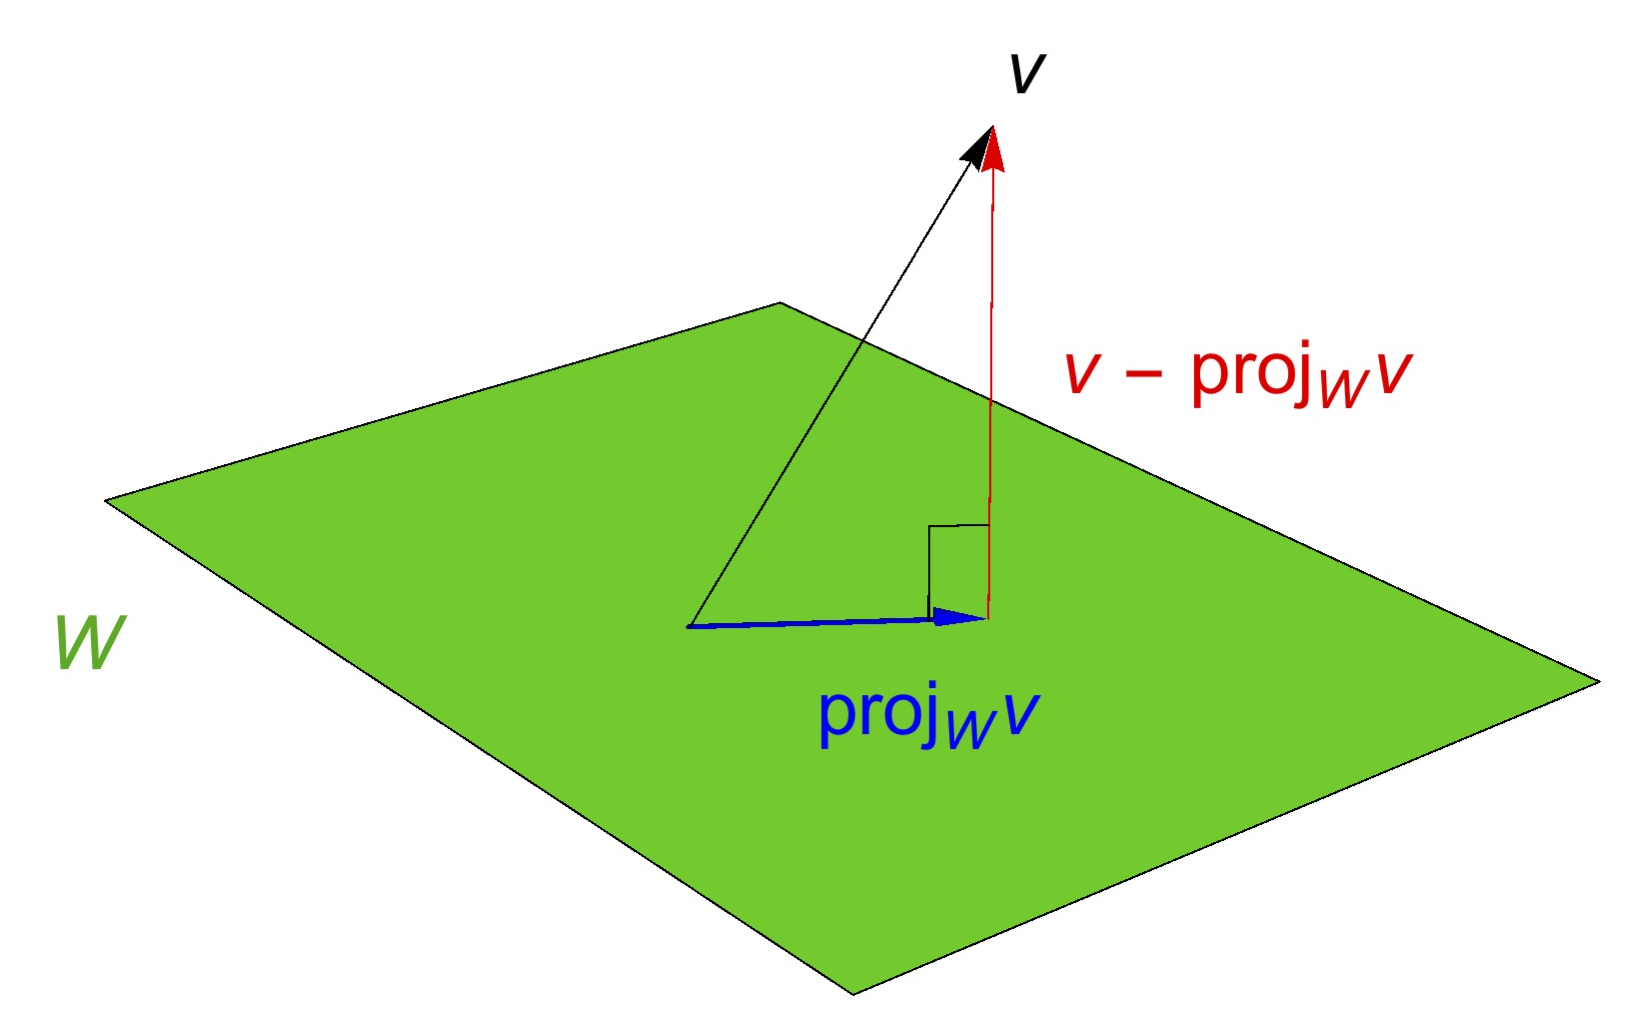
\includegraphics[scale=.2] {img/projW.jpg}~\\[1cm]
\end{center} 
\vglue-1cm
\caption{The orthogonal projection of $\vv$ onto the subspace $W$.}\label{figure:othogproj}
\end{figure}

Now your enquiring mind  may have at least two thoughts at this point. In no particular order, they may be:
\begin{enumerate}

\item {\it Does every subspace have an orthogonal basis?} The formula needs one!\label{goodquestion1}

\item {\it What if I compute this projection with two different orthogonal bases? Surely I'll get  different answers! All the numbers in the sum will be different...}
\end{enumerate}
 
\medskip

We'll answer the second question first -- it doesn't matter\footnote{Amazing fact from linear algebra number 3} which orthogonal basis you use! But not before an example.



\begin{myexample}
Let's look again at $W=\set{(x,y,z,w) \in \R^4 \st x-y-z+w=0}$. We know the three vectors  $\ww_1=(1,1,1,1), \ww_2=(1,-1,1,-1)$ and $ \ww_3=(1,1,-1,-1)$ form an orthogonal basis for $W$.\footnote{Don't worry about how we found these.   We'll discuss that later, in answer to the first question  above.}

Now   $\vv = (1,2,3,5) \notin W$: check it! Let's use the projection formula to find the orthogonal projection of $\vv$ onto $W$, and do a bit of checking.




\begin{mysol}  We begin by calculating:
$$
\frac{\vv\cdot \ww_1}{\|\ww_1\|^2} = \frac{11}{4} 
$$
$$
\frac{\vv\cdot \ww_2}{\|\ww_2\|^2} = \frac{-3}{4} 
$$
$$
\frac{\vv\cdot \ww_3}{\|\ww_3\|^2} = \frac{-5}{4}
$$

and conclude
$$
\proj_W(\vv) = \frac{11}4\ww_1 - \frac34\ww_2 - \frac{5}{4}\ww_3=\frac14(3, 9, 13, 19)
$$
 If you check, you'll see that  $\frac14(3, 9, 13, 19)\in W$: simply show it satsifies $x-y-z+w=0$. 

{\bf N.B. \underbar{You must not rescale this answer!} This is a very, very common error at this stage. Rescaling an orthogonal basis is fine, but the projection is a fixed answer.  }

Moreover, as Figure~\ref{figure:othogproj}, and indeed the properties of $\vv-\proj_W(\vv)$ in $\R^3$ (see Section~\ref{propOrthogProj}  and Figure~\ref{orthoprojonvector})
all suggest,  
$\vv-\proj_W(\vv)=\frac14(1, -1, -1, 1)$ is indeed orthogonal to every vector in $W$: look again at the equation defining $W$: it says $(x,y,z,w) \in W$ iff 
$$ 0=x-y-z+w=(x,y,z,w)\cdot(1, -1, -1, 1)!$$So every vector in $W$ {\it is} orthogonal to $\vv-\proj_W(\vv)$.
\end{mysol} 
\end{myexample}
\standout{This {\it always} happens. And as both Figures \ref{orthoprojonvector} and \ref{figure:othogproj} also suggest, this makes $\proj_W(\vv)$ {\it the \it closest vector in $W$ to $\vv$}. 

Another way to say this is that $\proj_W(\vv)$ is the {\it best approximation to $\vv$ by vectors in $W$}.}

Let's show that this is true:
\begin{theorem}[The Best Approximation Theorem]\index{orthogonal projection}\label{orthogproj}
Let $W$ be a subspace of $\R^n$ and let $\vv \in \R^n$. Then,

\begin{enumerate}[(1)]
\item $\proj_W(\vv) \in W$,
\item $\vv - \proj_W(\vv)$ is orthogonal to every vector in $W$,
\item $\proj_W(\vv)$ is best approximation to $\vv$ by vectors in $W$, and 
\item The vector $\proj_W(\vv)$ is the \underbar{only} vector in $\R^n$ which satisfies (1) and (2).
\end{enumerate} 

\end{theorem}

 

(Property 4 says that the orthogonal
projection is uniqely characterized by the two properties (1) and (2).)


\begin{proof} Part (1) is easy: look at the formula in Definition~\ref{projdef}. The vector $\proj_W(\vv)$ is a linear combination of vectors in the (subspace) $W$ and so must belong to $W$.

For (2), let's think: how {\it could} we  show 
a vector is orthogonal to every vector in $W$? There are infinitely many vectors in (most) subspaces! But that's one thing bases are very good for -- rendering finite  the infinite ! 

So suppose $\{\ww_1, \cdots, \ww_m\}$ is the orthogonal basis for $W$ we used to define the projection. Every $\uu\in W$ is a linear combination of $ \ww_1, \cdots, \ww_m $, \emph{i.e.}, $$\uu =a_1 \ww_1 +\cdots + a_m \ww_m$$ for some scalars $a_, \dots, a_m$. Set $\ww=\proj_W(\vv)$.  So if $(\vv-\proj_W(\vv))\cdot \ww_i=0$  for $1\le i \le m$, then $(\vv-\ww)\cdot \ww_i=0$ so
\begin{align*} 
(\vv-\ww) \cdot \uu &=(\vv-\ww)\cdot (a_1 \ww_1 +\cdots + a_m \ww_m) \\
&=a_1((\vv-\ww)\cdot \ww_1) +\cdots +a_1((\vv-\ww)\cdot \ww_m)\\
&=a_1(0) +\cdots +a_1(0)\\&=0.
\end{align*}
So, it suffices\footnote{Note that we did not use any property of $\{\ww_1, \cdots, \ww_m\}$ except that it spanned $W$, so the same computation shows that a vector is orthogonal to every vector in a subspace $W$ iff it is orthogonal to any {\it spanning set} of $W$.\label{CheckOrthogOnSpan} } to show that $(\vv-\ww)\cdot \ww_i=0$  for $1\le i \le m$.   So we calculate: 
\begin{align*}
 (\vv-\ww)\cdot\ww_i  &=
(\vv - (\frac{\vv\cdot \ww_1}{\Vert \ww_1\Vert^2}\ww_1 + \cdots 
+ 
\frac{\vv\cdot \ww_m}{\Vert \ww_m\Vert^2}\ww_m))\cdot \ww_i \\
 &= \vv \cdot \ww_i - \frac{\vv\cdot \ww_1}{\Vert \ww_1\Vert^2}\ww_1 \cdot \ww_i - \cdots - \frac{\vv\cdot \ww_m}{\Vert \ww_m\Vert^2}\ww_m \cdot \ww_i\\
&= \vv \cdot \ww_i - \frac{\vv\cdot \ww_i}{\Vert \ww_i\Vert^2}\ww_i \cdot \ww_i
\end{align*}

(since all the other dot products between $\ww_i$ and $\ww_j$ are zero);
and this last term gives
$$
 = \vv \cdot \ww_i - \frac{\vv\cdot \ww_i}{\Vert \ww_i\Vert^2}\Vert \ww_i \Vert^2 = 0.
$$
This is true for every $i = 1,2,\cdots, m$ so we conclude that $\vv-\ww$ is orthogonal to every vector in $W$, as required. This shows that (2) is true.


To show that (3) holds, denote, as before $\ww = \proj_W(\vv)$.  To prove this is the closest vector
in $W$ to $\vv$, let $\ww' \in W$ be any other vector in $W$.
Then
$$
\Vert \vv- \ww' \Vert^2 = \Vert (\vv - \ww) + (\ww - \ww') \Vert^2
$$
But since $\vv-\ww$ is orthogonal to every vector in $W$, and $\ww - \ww' \in W$ ($W$ is a subspace and both $\ww$ and $\ww'$ belong to $W$), the two vectors $ \vv - \ww$ and  $\ww - \ww'$
are orthogonal! So by the Pythagorean theorem \ref{eqn:Pythag} on P. \pageref{eqn:Pythag}, we have
$$
\Vert \vv- \ww' \Vert^2 = \Vert (\vv - \ww)\Vert^2 + \Vert(\ww - \ww') \Vert^2 \geq \Vert (\vv - \ww)\Vert^2,
$$
since $0\leq \Vert(\ww - \ww') \Vert^2$  is always true. Thus we've shown (3) is true.

The last part (4) is also straightforward. Now suppose two vectors $\ww,\ww'$ satisfy the properties (1) and (2) above, namely:

\begin{itemize}
\item $\ww, \ww' \in W$
\item $\vv - \ww$ and $\vv-\ww'$ are both orthogonal to every vector in $W$.
\end{itemize}

Then, $\ww- \ww'\in W$ since $W$, being a subspace, is closed under subtraction. But look: $$\ww- \ww'= (\vv-\ww')-(\vv - \ww).$$ Now the sum  -- or difference -- of two vectors which are both orthogonal to every vector in $W$ will again be orthogonal to every vector in $W$.\footnote{I don't know about you, but I'm getting tired of writing `is orthogonal to every vector in $W$', so soon we will save ourslves some bother and give a name to the collection of all vectors orthogonal to every vector in $W$. We'll call it $W^\perp$ --- see Chapter \ref{chapter:20OrthogComp}.} This means that the vector $\ww- \ww'$ is orthogonal to every vector in $W$, including $\ww- \ww'$ itself! But the only vector orthogonal to itself is the zero vector: so $\ww- \ww'=0$, i.e., $\ww= \ww'$.

This  shows that  there is only one vector with the  properties (1) and (2) above, namely $\proj_W(\vv)$.

\end{proof}

Note that  property (3) above of the orthogonal projection is extremely useful, in many areas. It is a huge part of the mathematical foundation for modern signal processing. It is used in almost all quantitative methods for `best' curve fitting for data. We present an example of this in Section~\ref{leastsquares}. 

\medskip

The basic idea it that we have often a `favourite' subspace of vectors $W$ (in a vector space of signals, for example), and another vector that we can't be sure belongs to our subspace, but we only wish to deal with vectors in $W$\kern-2pt, so we project our vector onto $W$ and deal with that instead. 

For example, in a simplified view of signal processing, on your cellphone, for example, when you take a picture and want to send it to a friend, the picture is captured and stored and treated as a vector in a large dimensional space ($\R^n$ for some very large $n$). But instead of sending all the data involved, it will be (orthogonally) projected onto a much smaller subspace -- with an  orthogonal basis peculiar to the protocol being used -- and then only the relatively small number (the dimension of $W$) of Fourier coefficients  will be transmitted. At the other end, your friend will receive the Fourier coefficients, and knowing which  protocol you used, will use the same  orthogonal basis, and rebuild the projection using the the Fourier coefficients, getting an approximation (better or worse, depending on $\dim W$) of the picture you sent.

\medskip

Part (4) above seems innocuous until you recall that Definition~\ref{projdef} {\it looked like} it depended on a choice of orthogonal basis. So what Part (4) is saying is that the {\it apparently} different formulae one gets when using different orthogonal bases to compute the projection all give exactly the same answer!

\section{Finding orthogonal bases: The Gram-Schmidt algorithm}\label{section:Gram-Schmidt}

So far, we've implicitly assumed that every subspace $W$ of $\R^n$ {\it has} an orthogonal basis. Is is true? Yes, and even better, there's a simple algorithm that will take any basis of $W$ as input and output an orthogonal basis of $W$. 

\medskip
 

Suppose  $\set{\uu_1, \cdots, \uu_m }$ is any basis for $W$.  We want to find an orthogonal
basis for $W$.

The geometric idea is quite simple:  start with your first vector $\uu_1$.
Then take $\uu_2 - \proj_{\uu_1}(\uu_2)$ to get something which is
orthogonal to $\uu_1$ but --- crucially --- lies in the span of $\uu_1$
and $\uu_2$.  We then keep subtracting off projections onto the span of the
preceding vectors we obtain and the result is an orthogonal basis for $W$.

\begin{theorem}[Gram-Schmidt Algorithm]\index{Gram-Schmidt algorithm}\label{theorem:GS}
Let $\set{\uu_1, \cdots, \uu_m }$ be {\it any} basis for $U$.  Define
\begin{itemize}
\item $\ww_1 = \uu_1$  and $V_1 = \spn\{\ww_1\}$
\item $\ww_2 = \uu_2 - \proj_{V_1}\uu_2$ and $V_2 = \spn\{\ww_1,\ww_2\}$
\item $\ww_3 = \uu_3 - \proj_{V_2}\uu_3$ and $V_3 = \spn\{\ww_1,\ww_2,\ww_3\}$
\item $\cdots$
\item $\ww_m = \uu_m - \proj_{V_{m-1}}\uu_m$ and $V_m = \spn\{\ww_1,\cdots,\ww_m\}$
\end{itemize}
Then $W = V_m$ and   
$\{\ww_1,\cdots,\ww_m\}$ is an orthogonal basis for $W$.

\medskip
Written out in more detail: define

\begin{itemize}
\item $\ww_1 = \uu_1$,
\item $\ww_2 = \uu_2 - \proj_{\ww_1}\ww_2$,
\item $\ww_3 = \uu_3 - \proj_{\ww_1}\uu_3-\proj_{\ww_2}\uu_3$,
\item $\cdots$
\item $\ww_m = \uu_m - \sum_{i=1}^{m-1}\proj_{\ww_{i}}\uu_m$.
\end{itemize}
Then $\{\ww_1,\cdots,\ww_m\}$ is an orthogonal basis for $U$.

Finally, one could scale each of the  vectors $\ww_i$ by dividing by their norm to produce
an  orthonormal basis for $W$.
\end{theorem}

Notice that at each step, the vectors in the spanning set for $V_i$
are orthogonal, so that means it's easy to calculate the projection onto
$V_k$.  And in fact, $V_k = \spn\{\uu_1 , \cdots, \uu_k\}$; that is, the span of the first
$k$ vectors of the set is the same as the span of the first $k$
vectors of the original spanning set.  

\medskip
Indeed, one could begin with just a {\it spanning} set $\set{\uu_1,\dots, \uu_n}$ for $U$, and apply the Gram-Schmidt Algorithm as above: then the {\it non-zero} vectors in $\{\ww_1,\cdots,\ww_n\}$ would be an orthogonal basis for $U$ - see problem~\ref{prob19.6} in the exercises.

\begin{myexample}\label{example:GS} Let's perform the Gram-Schmidt algorithm on the 
the set
$$\{ (1,0,0,1), (1,1,1,0), (2,1,-1,1)\}
$$
(You can check that this is a basis for the subspace $W=\spn\{ (1,0,0,1), (1,1,1,0), (2,1,-1,1)\}=\set{(x,y,z,w)\in \R^4\st x - y - w = 0}$.\footnote{We saw how to do this at the end of chapter \ref{chapter:15homog}.})


Well, we start with 
$$
\ww_1 = (1,0,0,1)
$$
and then
\begin{align*}
\ww_2 &= \uu_2 - \proj_{\ww_1}\uu_2\\
&= \uu_2 - \frac{\uu_2\cdot \ww_1}{\|\ww_1\|^2}\ww_1 \\
&= (1,1,1,0) - \frac{1}{2}(1,0,0,1) = (\frac12,1,1,-\frac12). 
\end{align*}
(Before going on, it's always a good idea to check that $\ww_1\cdot \ww_2 =0$! It's OK here.)

So in this example, there's just one more step:

\begin{align*}
\ww_3 &= \uu_3 - \frac{\uu_3\cdot \ww_1}{\|\ww_1\|^2}\ww_1 - \frac{\uu_3\cdot \ww_2}{\|\ww_2\|^2}\ww_2\\
&= (2,1,-1,1) - \frac{3}{2} (1,0,0,1) - \frac{\frac12}{\frac52}
(\frac12,1,1,-\frac12) \\
&= (2,1,-1,1) -(\frac32,0,0,\frac32) - (\frac1{10}, \frac15
 , \frac15, -\frac1{10})\\
&= \frac25(1, 2 , -3 , -1).
\end{align*}
Then we can see that $\{\ww_1,\ww_2,\ww_3\}$ is indeed orthogonal -- and it's always a good idea to check this.\footnote{If you can, it's also a very good idea to check that your vectors $\{\ww_1,\ww_2,\ww_3\}$ belong to $W$-- which of course they should! In this case that's easy, as we have a simple description of $W$ -- namely, $W=\set{(x,y,z,w)\in \R^4\st x - y - w = 0}$.}  Also,
by looking at our calculations more carefully, we can see that indeed,
each successive element is in the span of the original vectors. 
The resulting orthogonal basis is
$$
\{ (1,0,0,1), \frac12(1,2,2,-1), \frac25(1,2,-3,-1)\}.
$$  

\begin{remark} We often choose to simplify our calculations when using the formula in Theorem~\ref{theorem:GS} by scaling the 
$\ww_i$ by something convenient to avoid fractions: since 
$$
\{ (1,0,0,1), (1,2,2,-1), (1,2,-3,-1)\}
$$
is just as good an orthogonal set as the one above, and might be
easier to work with if you had to calculate another projection.
\end{remark}

\medskip
Finally, if one really wants  an orthonormal basis, we have to divide each 
of these vectors by their norm.  Since 
$
\Vert (1,0,0,1) \Vert = \sqrt{2}$,  $\Vert  (1,2,2,-1) \Vert =   \sqrt{10}$, and $ \Vert  (1,2,-3,-1) \Vert =   \sqrt{15} $, we obtain the orthonormal basis:
$$
\{ \frac{\sqrt{2}}{2}(1,0,0,1), \frac{\sqrt{10}}{ 10 }(1,2,2,-1), \frac{\sqrt{15}}{15}(1,2,-3,-1)\}.
$$
(Check this!)
\end{myexample}



\begin{myexample}\label{Wagain} Calculate the best approximation to  $\vv = (1,2,3,4)$ in $W$, where
$$
W = \spn\{(1,0,0,1), (1,1,1,0), (2,1,-1,1)\}=\set{(x,y,z,w)\in \R^4\st x - y - w = 0}
$$

Let's use the preceding exercise.  We already know that an
orthogonal basis for $W$ is 
$$
\{  (1,0,0,1),  (1,2,2,-1),  (1,2,-3,-1)\}
$$
(call these $\nn_1$, $\nn_2$ and $\nn_3$, say)
so therefore 
\begin{align*}
\proj_W(\vv) &= \frac{\vv\cdot\nn_1}{\|\nn_1\|^2} \nn_1 +  \frac{\vv\cdot\nn_2}{\|\nn_2\|^2} \nn_2 + \frac{\vv\cdot\nn_3}{\|\nn_3\|^2} \nn_3 \\  
&= \frac{5}{2}  (1,0,0,1) + \frac{7}{10} (1,2,2,-1)  -\frac{8}{15}(1,2,-3,-1)\\
&=  \frac{1}{3}(8,1,3,7).
\end{align*}

If you can, check that your answer actually belongs to $W$: here it's easy since we have a simple description of $W$.\footnote{ If you have the time, you should also check that $(1,2,3,4)-\frac{1}{3}(8,1,3,7)=\frac13(-5,5,0,5)$ is orthogonal to everything in $W$, and it is, since $\frac13(-5,5,0,5).(x,y,z,w)=-\frac53 (x-y-w)=0 $ whenever $(x,y,z,w)\in W$! }
\end{myexample}


